\documentclass[../../main.tex]{subfiles}

\begin{document}
\graphicspath{{img/}{05_software/img/}}

\chapter{Implement Gmapping trên nền tảng CUDA}


Bài toán: Giả sử có $N$ particles, mỗi particle biểu diễn một trạng thái của robot bao gồm tọa độ x,y, góc quay theta $(x, y, \theta)^T$ và một map $m_n$ tương ứng với trạng thái đó. Với mỗi bộ dữ liệu đầu vào bao gồm ranging data và odometry data, ta cần dự đoán trạng thái mới của robot đồng thời tiếp tục cập nhật map của môi trường xung quanh.

Nội dung chương phân tích quá trình implement GMapping để giải quyết bài toán trên theo các bước cơ bản của Particle Filter.

\section{Dự đoán - Prediction}
Ở bước này, trạng thái tiếp theo của các particle được tính dựa vào motion model cung cấp từ odometry system. 
\begin{equation}
    \begin{pmatrix}
        \hat{x} \\ \hat{y} \\ \hat{\theta}
    \end{pmatrix}
    = 
    \begin{pmatrix}
        x \\ y \\ \theta
    \end{pmatrix}
    + 
    \begin{pmatrix}
        dx \\ dy \\ d\theta
    \end{pmatrix}
\end{equation}
Với $dx$, $dy$, $d\theta$ có được bằng cách lấy hiệu của trạng thái cung cấp từ odometry hiện giờ và vòng lặp trước.

\section{Hiệu chỉnh - Correction}
Particle filter không có bước này nhưng nó lại giữ một vai trò quan trọng để tăng độ chính xác của thuật toán, nhất là khi có nhiều nhiễu trong quá trình di chuyển của mobile robot hoặc tần số  chạy thuật toán thấp.

Để thực hiện corection, ta sử dụng thuật toán IPC (iterative closest point). Một cách ngắn gọn có thể mô tả thuật toán này như sau:
\begin{itemize}
    \item Với vị trí hiện tại của robot, ta tính toán vị trí của các điểm cuối (vị trí mà các tia laser va vào vật) từ ranging data.
    \item Với mỗi điểm cuối, ta tìm một điểm tương ứng trên map
    \item Sử dụng công thức để tìm biến đổi trung bình từ tập các điểm cuối đến các điểm tương ứng trên map.
    \item Áp dụng phép biến đổi đó vào vị trí hiện tại của robot ta được vị trí mới.
    \item Tiếp tục quay lại bước đầu cho đến khi vị trí robot hầu như không thay đổi nữa hoặc quá một số lượng vòng lặp giới hạn nhất định.
\end{itemize}

Có nhiều cách để tìm điểm tương ứng: điểm gần nhất, điểm gần nhất theo trục x, theo trục y,... Tuy nhiên để đạt được kết quả tốt nhất, ta nên sử dụng thuật toán Bresenham để tìm điểm tương ứng thuộc map trên đường thẳng nối từ vị trí của robot tới điểm cuối.

\section{Tính weight cho từng particle - Scoring}
Với mỗi particle, ta tính weight dựa vào sự tương đồng giữa các điểm cuối tính từ ranging data và vị trí của robot so với các điểm tương ứng trên map. Việc tìm điểm tương đồng sử dụng thuật toán Bresenham.

Giả sử  ta có $M$ điểm cuối $(x_i^r, y_i^r)^T$ và $M$ điểm tương ứng trên map $(x_i^m, y_i^m)^T$, weight cho mỗi particle được tính theo công thức:
\begin{equation}
    w_i = \frac{m}{\exp((x_i^r-x_i^m)^2 + (y_i^r - y_i^m)^2)}
\end{equation}
Với $m$ là xác suất mà ô có vị trí $(x_i^m, y_i^m)^T$ trên map bị chiếm dụng.

\section{Lấy mẫu lại - Resampling}
Việc lấy mẫu lại có mục đích làm tăng sự xuất hiện của các particle có weight cao đồng thời làm giảm hoặc biến mất các particle có trọng số thấp.
Thuật toán multinomial resampling được sử dụng để lấy mẫu lại các particle.

\begin{figure}[ht]
    \begin{center}
        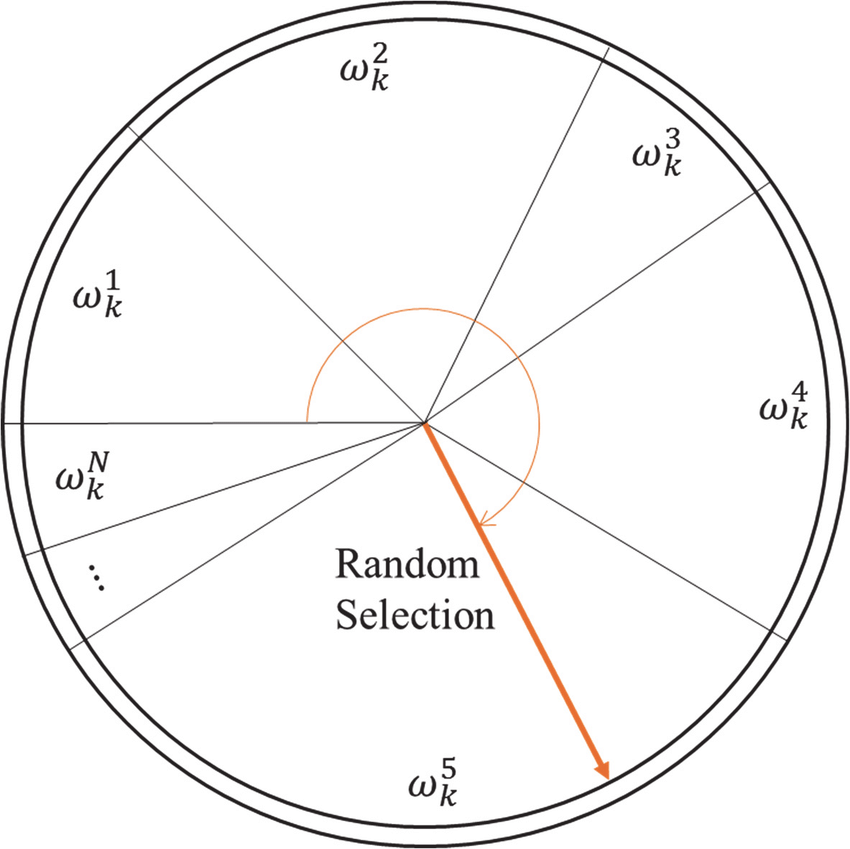
\includegraphics[scale=0.2]{Visualization-of-multinomial-resampling-algorithm.png}
    \end{center}
    \caption{Mô tả hình học của thuật toán multinomial resampling}
    \label{fig:Visualization-of-multinomial-resampling-algorithm}
\end{figure}

Multinomial resampling bao gồm các bước sau:
\begin{itemize}
    \item Chuẩn hóa cái giá trị weight
    \item Tính tổng tính lũy các weight
    \item Lấy mẫu ngẫu nhiên $N$ số  có khoảng giá trị từ 0 đến 1 theo phân phối đều
    \item Với mỗi mẫu lấy được, xác định vị trí của weight mà nó thuộc về và lấy mẫu particle tương ứng với weight đó. VD: trong hình \ref{fig:Visualization-of-multinomial-resampling-algorithm}, mẫu màu cam nằm trong vị trí của $w^5$ nên particle có weight là $w^5$ được lấy mẫu.
\end{itemize}
\end{document}